%%%%%%%%%%%%%%%%%%%%%%%%%%%%%%%%%%%%%%%%%
% University/School Laboratory Report
% LaTeX Template
% Version 3.1 (25/3/14)
%
% This template has been downloaded from:
% http://www.LaTeXTemplates.com
%
% Original author:
% Linux and Unix Users Group at Virginia Tech Wiki 
% (https://vtluug.org/wiki/Example_LaTeX_chem_lab_report)
%
% License:
% CC BY-NC-SA 3.0 (http://creativecommons.org/licenses/by-nc-sa/3.0/)
%
%%%%%%%%%%%%%%%%%%%%%%%%%%%%%%%%%%%%%%%%%

%----------------------------------------------------------------------------------------
%	PACKAGES AND DOCUMENT CONFIGURATIONS
%----------------------------------------------------------------------------------------

\documentclass{article}

\usepackage[version=3]{mhchem} % Package for chemical equation typesetting
%\usepackage{siunitx} % Provides the \SI{}{} and \si{} command for typesetting SI units
\usepackage{graphicx} % Required for the inclusion of images
\usepackage{natbib} % Required to change bibliography style to APA
\usepackage{amsmath} % Required for some math elements 
\usepackage{hyperref}
\usepackage[a4paper,margin=0.5in]{geometry}
\setlength\parindent{0pt} % Removes all indentation from paragraphs

\renewcommand{\labelenumi}{\alph{enumi}.} % Make numbering in the enumerate environment by letter rather than number (e.g. section 6)

%\usepackage{times} % Uncomment to use the Times New Roman font

%----------------------------------------------------------------------------------------
%	DOCUMENT INFORMATION
%----------------------------------------------------------------------------------------

\title{Gate Detection} % Title

\author{Philipp \textsc{Duernay}} % Author name

\date{\today} % Date for the report

\begin{document}
\maketitle
% If you wish to include an abstract, uncomment the lines below
% \begin{abstract}
% Abstract text
% \end{abstract}

%----------------------------------------------------------------------------------------
%	SECTION 1
%----------------------------------------------------------------------------------------

\section{Recap}
In the last meeting from 28.03.2018 several next steps were defined:
\begin{enumerate}
	\item \textbf{Generate data with Airsim}
	\item \textbf{Compare performance when gate contains an image}
	\item \textbf{Use ssd from tensorflow-object-detection api}
	\item \textbf{Rethink approach, How to define an object?}
\end{enumerate}

\section{Data Generation}
Getting ground truth bounding boxes out of the simulator took a bit more time than expected since this is not provided by default and how the graphic engine renders the scene is not very well documented. However, in the end ground truth labels could be obtained. A scene was created for training and testing the models. A screenshot is shown in \autoref{fig:scene}
\begin{figure}
	\begin{minipage}{0.5\textwidth}
		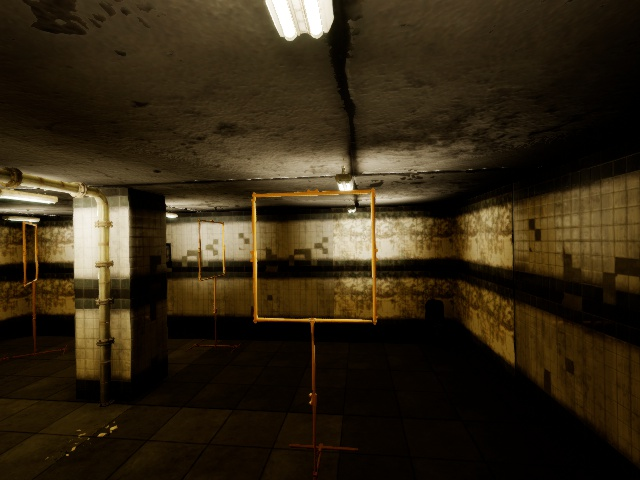
\includegraphics[width=\textwidth]{fig/industrial}
		\caption{Scene for training and testing models}
			\label{fig:scene}
	\end{minipage}
	\begin{minipage}{0.5\textwidth}
	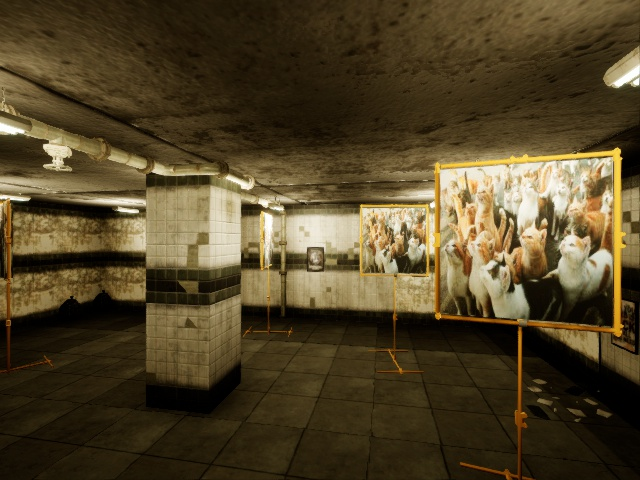
\includegraphics[width=\textwidth]{fig/industrial_cats}
		\caption{An example for gates with image}
		\label{fig:cats}
	\end{minipage}

\end{figure} 

\section{Evaluation}
We assume the reason for the low performance so far is the absence of higher order features. Deep object detectors like Yolo rely on the assumption that the lower layers with a small receptive field detect basic shapes like edges and corners, while higher layers combine those shapes in a deeper and deeper semantic representation. However, the object we want to detect basically consists of 4 corners and 4 lines in orange colour, whereas the biggest part of the bounding box that surrounds the object is occupied by background. 

In order to proof this hypothesis we do an experiment. We place an image with a more complex object inside the area that is occupied by background. Ideally the image itself is not too easy to detect such that the model has to learn a deeper representation. An example of the chosen image can be seen in \autoref{fig:cats}.

We train two models with and without the added image and compare their performance. In both cases the training set consists of 10 000 images. These are taken by placing the camera randomly within a certain space in the room. The arrangement of gates is changed 5 times so each batch of 2000 images sees the same arrangement of gates only from different angles. It has been taken care that the average number of gates within an image is larger than 1 (~1.4) to avoid too many negatives. The placement of the camera should be how a real drone would see the gates however with the current setup in the simulator it can't be fully avoided that the camera ends up "within" a wall sometimes.

For the testset the gates are placed like a race court. Then the camera is "flewn" manually through the course while images are recorded. The sets consists of 100 images each. Results can be seen in \autoref{fig:tiny} and \autoref{fig:v2}.

\begin{figure}
	\centering
	\begin{minipage}{0.4\textwidth}
		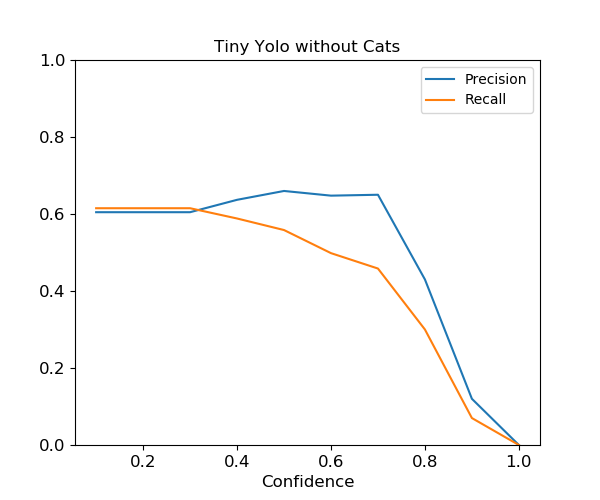
\includegraphics[width=\textwidth]{fig/pr_tiny}
	\end{minipage}
	\begin{minipage}{0.4\textwidth}
		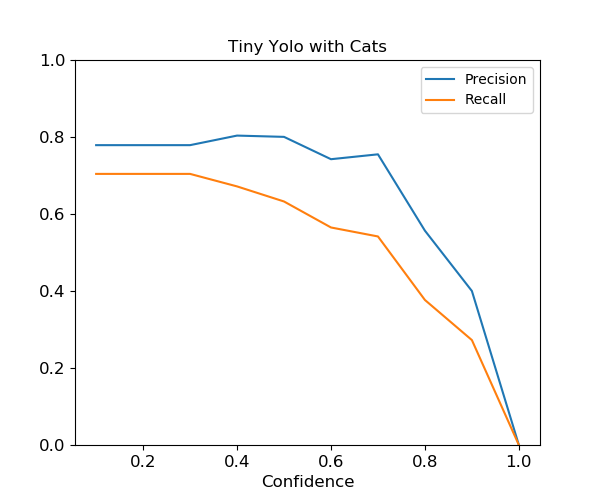
\includegraphics[width=\textwidth]{fig/pr_tiny_cats}
	\end{minipage}
	\begin{minipage}{0.4\textwidth}
	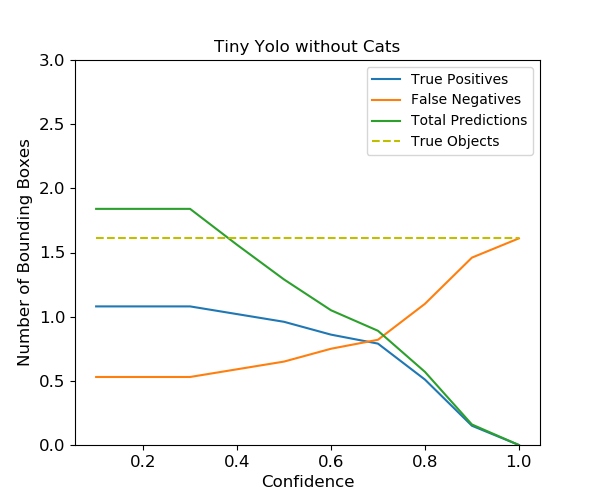
\includegraphics[width=\textwidth]{fig/detections_tiny}
	\end{minipage}
	\begin{minipage}{0.4\textwidth}
		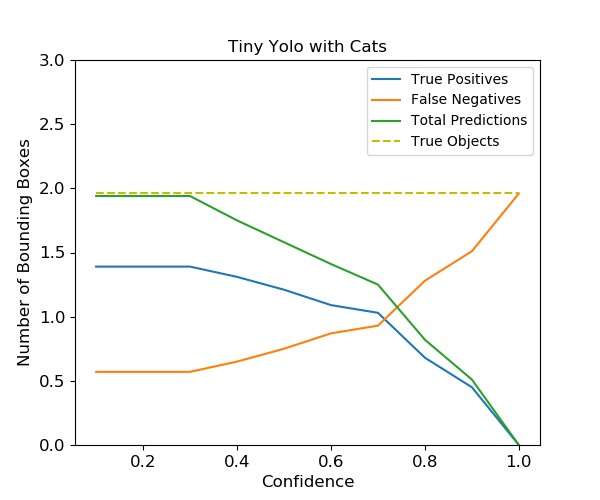
\includegraphics[width=\textwidth]{fig/detections_tiny_cats}
	\end{minipage}
	\caption{Performance of the Tiny Yolo model compared. The plots show an average value per image.}
	\label{fig:tiny}
\end{figure} 

\begin{figure}
	\centering
	\begin{minipage}{0.4\textwidth}
		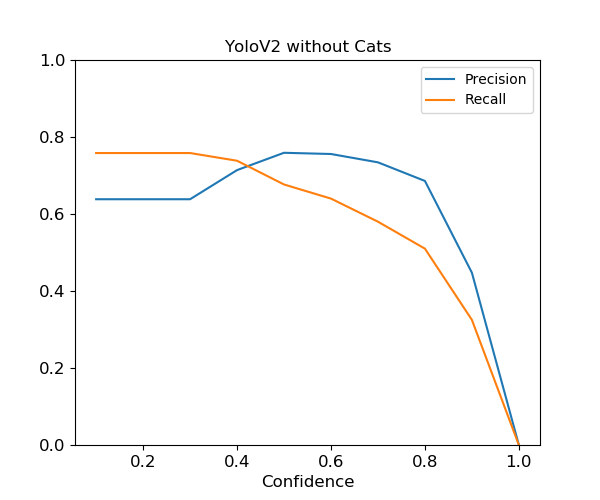
\includegraphics[width=\textwidth]{fig/pr_v2}
	\end{minipage}
	\begin{minipage}{0.4\textwidth}
		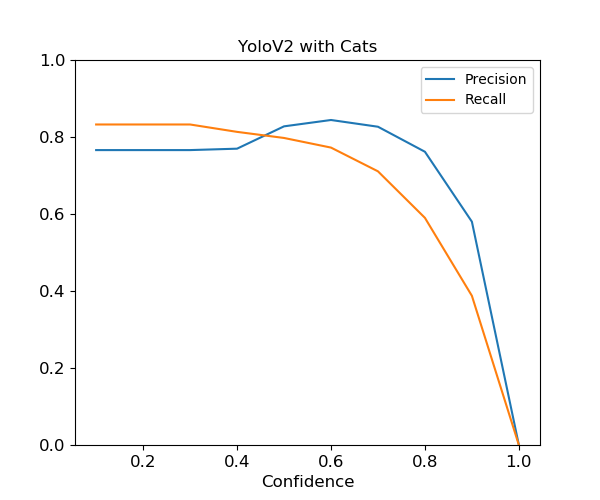
\includegraphics[width=\textwidth]{fig/pr_v2_cats}
	\end{minipage}
	\begin{minipage}{0.4\textwidth}
		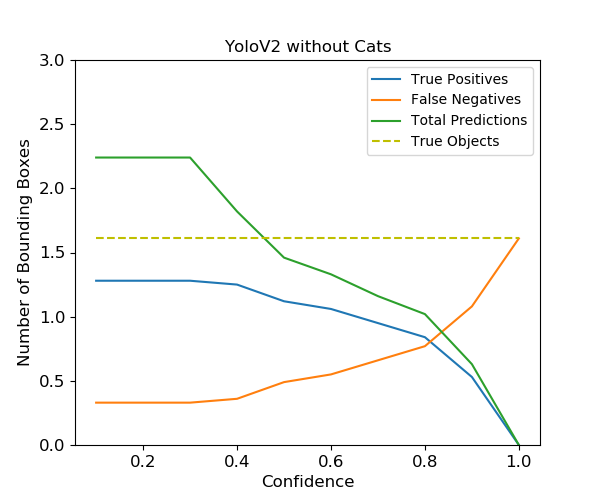
\includegraphics[width=\textwidth]{fig/detections_v2}
	\end{minipage}
	\begin{minipage}{0.4\textwidth}
		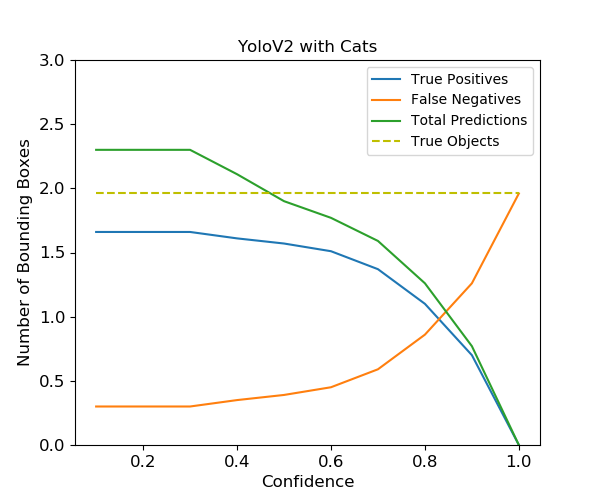
\includegraphics[width=\textwidth]{fig/detections_v2_cats}
	\end{minipage}
		\caption{Performance of the YoloV2 model compared. The plots show an average value per image.}
			\label{fig:v2}
\end{figure} 

Generally, we see poor performance of the yolo models on the simulated data. Even the deep model with 23 layers in best case gets a precision of 0.7 at a recall of 0.4. As a positive result one can see the fact that the absolute average amount of predictions/false positives is not insanely high. 

In \autoref{fig:examples} some examples are shown. We see how the model often predicts numerous boxes along one edge of the gate, while not predicting the true surrounding box accurately. It almost seems as if the model predicts a box somewhere as soon as it sees a orange edge somewhere without really taking the edges into account.

\begin{figure}
	\centering
	\begin{minipage}{0.3\textwidth}
		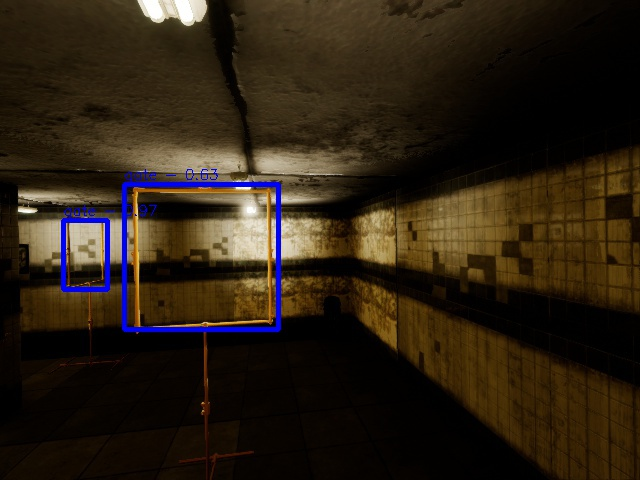
\includegraphics[width=\textwidth]{fig/v2}
	\end{minipage}
	\begin{minipage}{0.3\textwidth}
		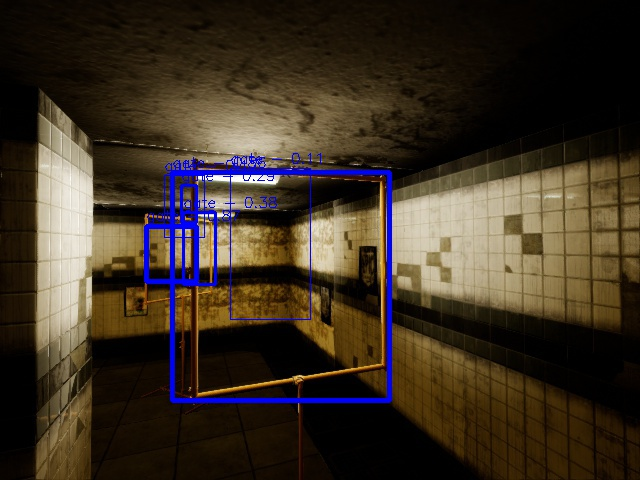
\includegraphics[width=\textwidth]{fig/v22}
	\end{minipage}
	\begin{minipage}{0.3\textwidth}
		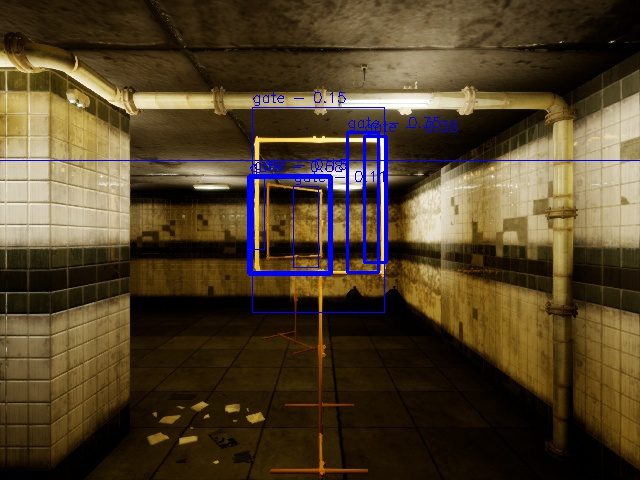
\includegraphics[width=\textwidth]{fig/v23}
	\end{minipage}
	\caption{YoloV2}
	\label{fig:examples}
\end{figure}

Within our experiment we see what we expected. The performance increases significantly when placing an image inside the gate. However, even then the best result is at a precision/recall of 0.8/0.8 only. The reason gets more clear when looking at actual images like \autoref{fig:examples_cat}. We see how the model fails when gates are only seen from the side. Here the model predicts multiple bounding boxes thereby ruining the precision. This makes sense as we now have the similar problem as before, there are almost no features to use. Another example was found (third image) where the gate was not detected at all although it is clearly visible. However, this is a rare case on most other images the gate gets detected accurately.

 
\begin{figure}
	\centering
	\begin{minipage}{0.3\textwidth}
		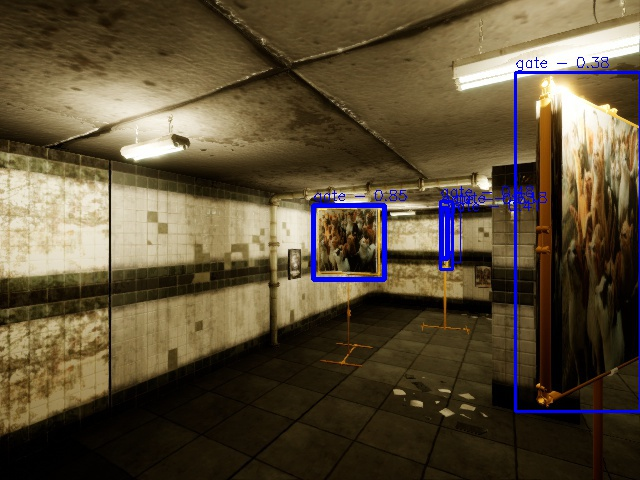
\includegraphics[width=\textwidth]{fig/v2_cats}
	\end{minipage}
	\begin{minipage}{0.3\textwidth}
		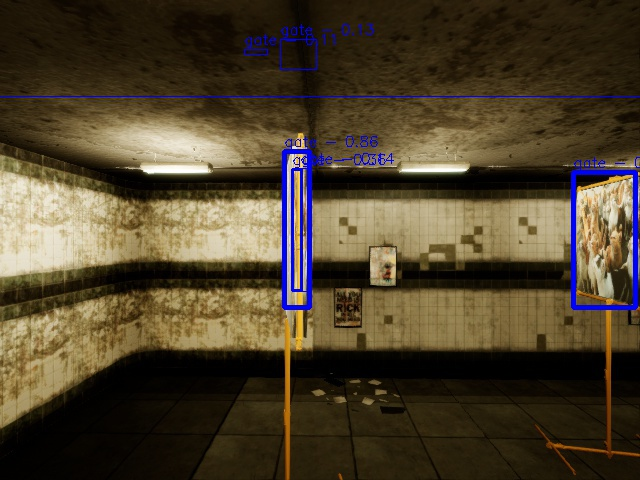
\includegraphics[width=\textwidth]{fig/v2_cat2}
	\end{minipage}
	\begin{minipage}{0.3\textwidth}
		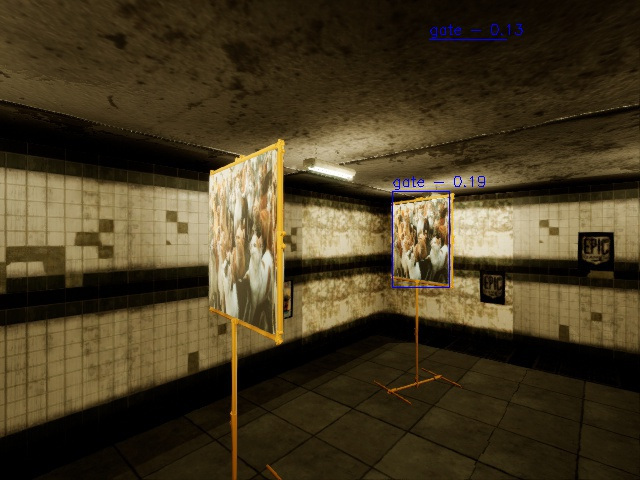
\includegraphics[width=\textwidth]{fig/v2cats3}
	\end{minipage}
	\caption{YoloV2}
	\label{fig:examples_cat}
\end{figure} 
\newpage
\section{Conclusion}

\begin{itemize}
	\item Results of yolo on the simulated data are not satisfying.
	\item The model seems to predict numerous boxes as soon as it sees an orange edge.
	\item The experiment of placing an image within the gates confirmed our assumption.
\end{itemize}

\section{Next Step}
\begin{itemize}
	\item Repeat Experiment with SSD
	\item Evaluate other models:
	\begin{itemize}
		\item Viola and Jones
		\item Deformable Parts: Model corners, pole 
		\item Custom CNN: Output as offset of default box in corner coordinates, Max Pooling with larger strides
		\item small cnn
		\item limit angles
	\end{itemize} 
\end{itemize}
%----------------------------------------------------------------------------------------


%----------------------------------------------------------------------------------------
%	BIBLIOGRAPHY
%----------------------------------------------------------------------------------------

\bibliographystyle{abbrv}

\bibliography{literature}

%----------------------------------------------------------------------------------------


\end{document}\grid
